\PassOptionsToPackage{table}{xcolor}
\documentclass{article}
\usepackage{iclr2027_conference,times}
\usepackage[T1]{fontenc}
\usepackage{wrapfig}
\usepackage{amsmath,amssymb,amsfonts,mathtools,amsthm}
\usepackage{booktabs,graphicx,multirow,makecell,tabularx}
\usepackage{capt-of}
\usepackage{float}
\usepackage{dblfloatfix}
\usepackage{xcolor}
\usepackage{microtype}
\usepackage{enumitem}
\usepackage{etoolbox}
\usepackage{placeins}
\usepackage{hyperref}
\hypersetup{hidelinks}
\usepackage{url}
\usepackage[nameinlink,capitalize,noabbrev]{cleveref}

% Compact float spacing for a dense conference-paper layout.
\setlength{\textfloatsep}{6pt plus 1.5pt minus 1.5pt}
\setlength{\floatsep}{5pt plus 1.5pt minus 1.5pt}
\setlength{\intextsep}{2pt}
\setlength{\abovecaptionskip}{4pt}
\setlength{\belowcaptionskip}{2pt}
% Keep tables compact while preserving a small, consistent gap before the
% following text.  The padding lives inside the float, so it follows the table
% even when LaTeX moves the float to the top of another page.
\AtEndEnvironment{table}{\vspace{3pt}}
\AtEndEnvironment{table*}{\vspace{3pt}}

% Submission mode: keep \iclrfinalcopy commented to preserve anonymity and
% line numbers. Do not modify iclr2027_conference.sty.
% \iclrfinalcopy

\newcommand{\pfdnav}{\textsc{P4D-Nav}}
\newcommand{\pfdbench}{\textsc{P4D-Bench}}
\newcommand{\evolvingworldnav}{\textsc{EvolvingWorldNav}}
\newcommand{\na}{--}
\definecolor{tblheader}{RGB}{233,238,245}
\definecolor{tblours}{RGB}{238,240,242}
\definecolor{tblreported}{RGB}{244,246,250}
\definecolor{tblnav}{RGB}{248,242,229}
\definecolor{tblmemory}{RGB}{232,241,249}
\definecolor{tblpredict}{RGB}{242,237,248}
\newcommand{\hdr}[1]{\colorbox{tblheader}{\strut #1}}

\title{EvolvingWorldNav: Predictive 4D Belief for Persistent Navigation in Evolving Worlds}

% ICLR 2027 is double blind. Author identities must not appear in either the
% paper or supplementary material until the camera-ready stage.
\author{Anonymous authors}

\begin{document}
\maketitle

\begin{abstract}
Long-lived embodied agents must navigate in evolving environments where object
locations can change outside their view, making accurate memories stale and
current-state inference from intermittent observations uncertain. Recent work
on persistent memory and open-vocabulary mapping supports retrieval of past
spatial experience, while predictive scene representations and routine models
learn temporal regularities in object states and placements. A remaining
challenge is to turn these predictions into physical decisions that retain
alternative hypotheses and gather reliable evidence as the world continues to
evolve during navigation. To address this challenge, we introduce
\evolvingworldnav{}, an embodied agent
that turns timestamped 3D entity histories into a belief over current object
locations. Our key insight is to separate whether the last observed state
remains valid from where the object may have moved, and to carry this
uncertainty through navigation rather than committing to a stale destination.
A continuous-time Transformer predicts this persistence--relocation belief
from irregular observations. The agent then balances candidate probability
against inspection cost and updates its belief during navigation using
visibility-aware evidence, distinguishing an empty location from an
inconclusive view. The learned predictor operates within a frozen
vision--language control loop. We also introduce \pfdbench{}, a
human-trace-grounded simulation benchmark with \textbf{54} scenes and
\textbf{803.68k} task instances for evaluating inference and action under
hidden world evolution. On its navigation evaluation, \evolvingworldnav{}
achieves \textbf{61.32\%} first-attempt success and \textbf{86.18\%} search
success, exceeding the strongest evaluated baseline by \textbf{15.99} and
\textbf{5.18} percentage points, respectively. Controlled evaluations show
that the predictive advantage is largest under learnable temporal structure,
motivating explicit uncertainty and evidence gathering when history alone is
insufficient.
\end{abstract}

\raggedbottom
\begin{figure}[H]
    \centering
    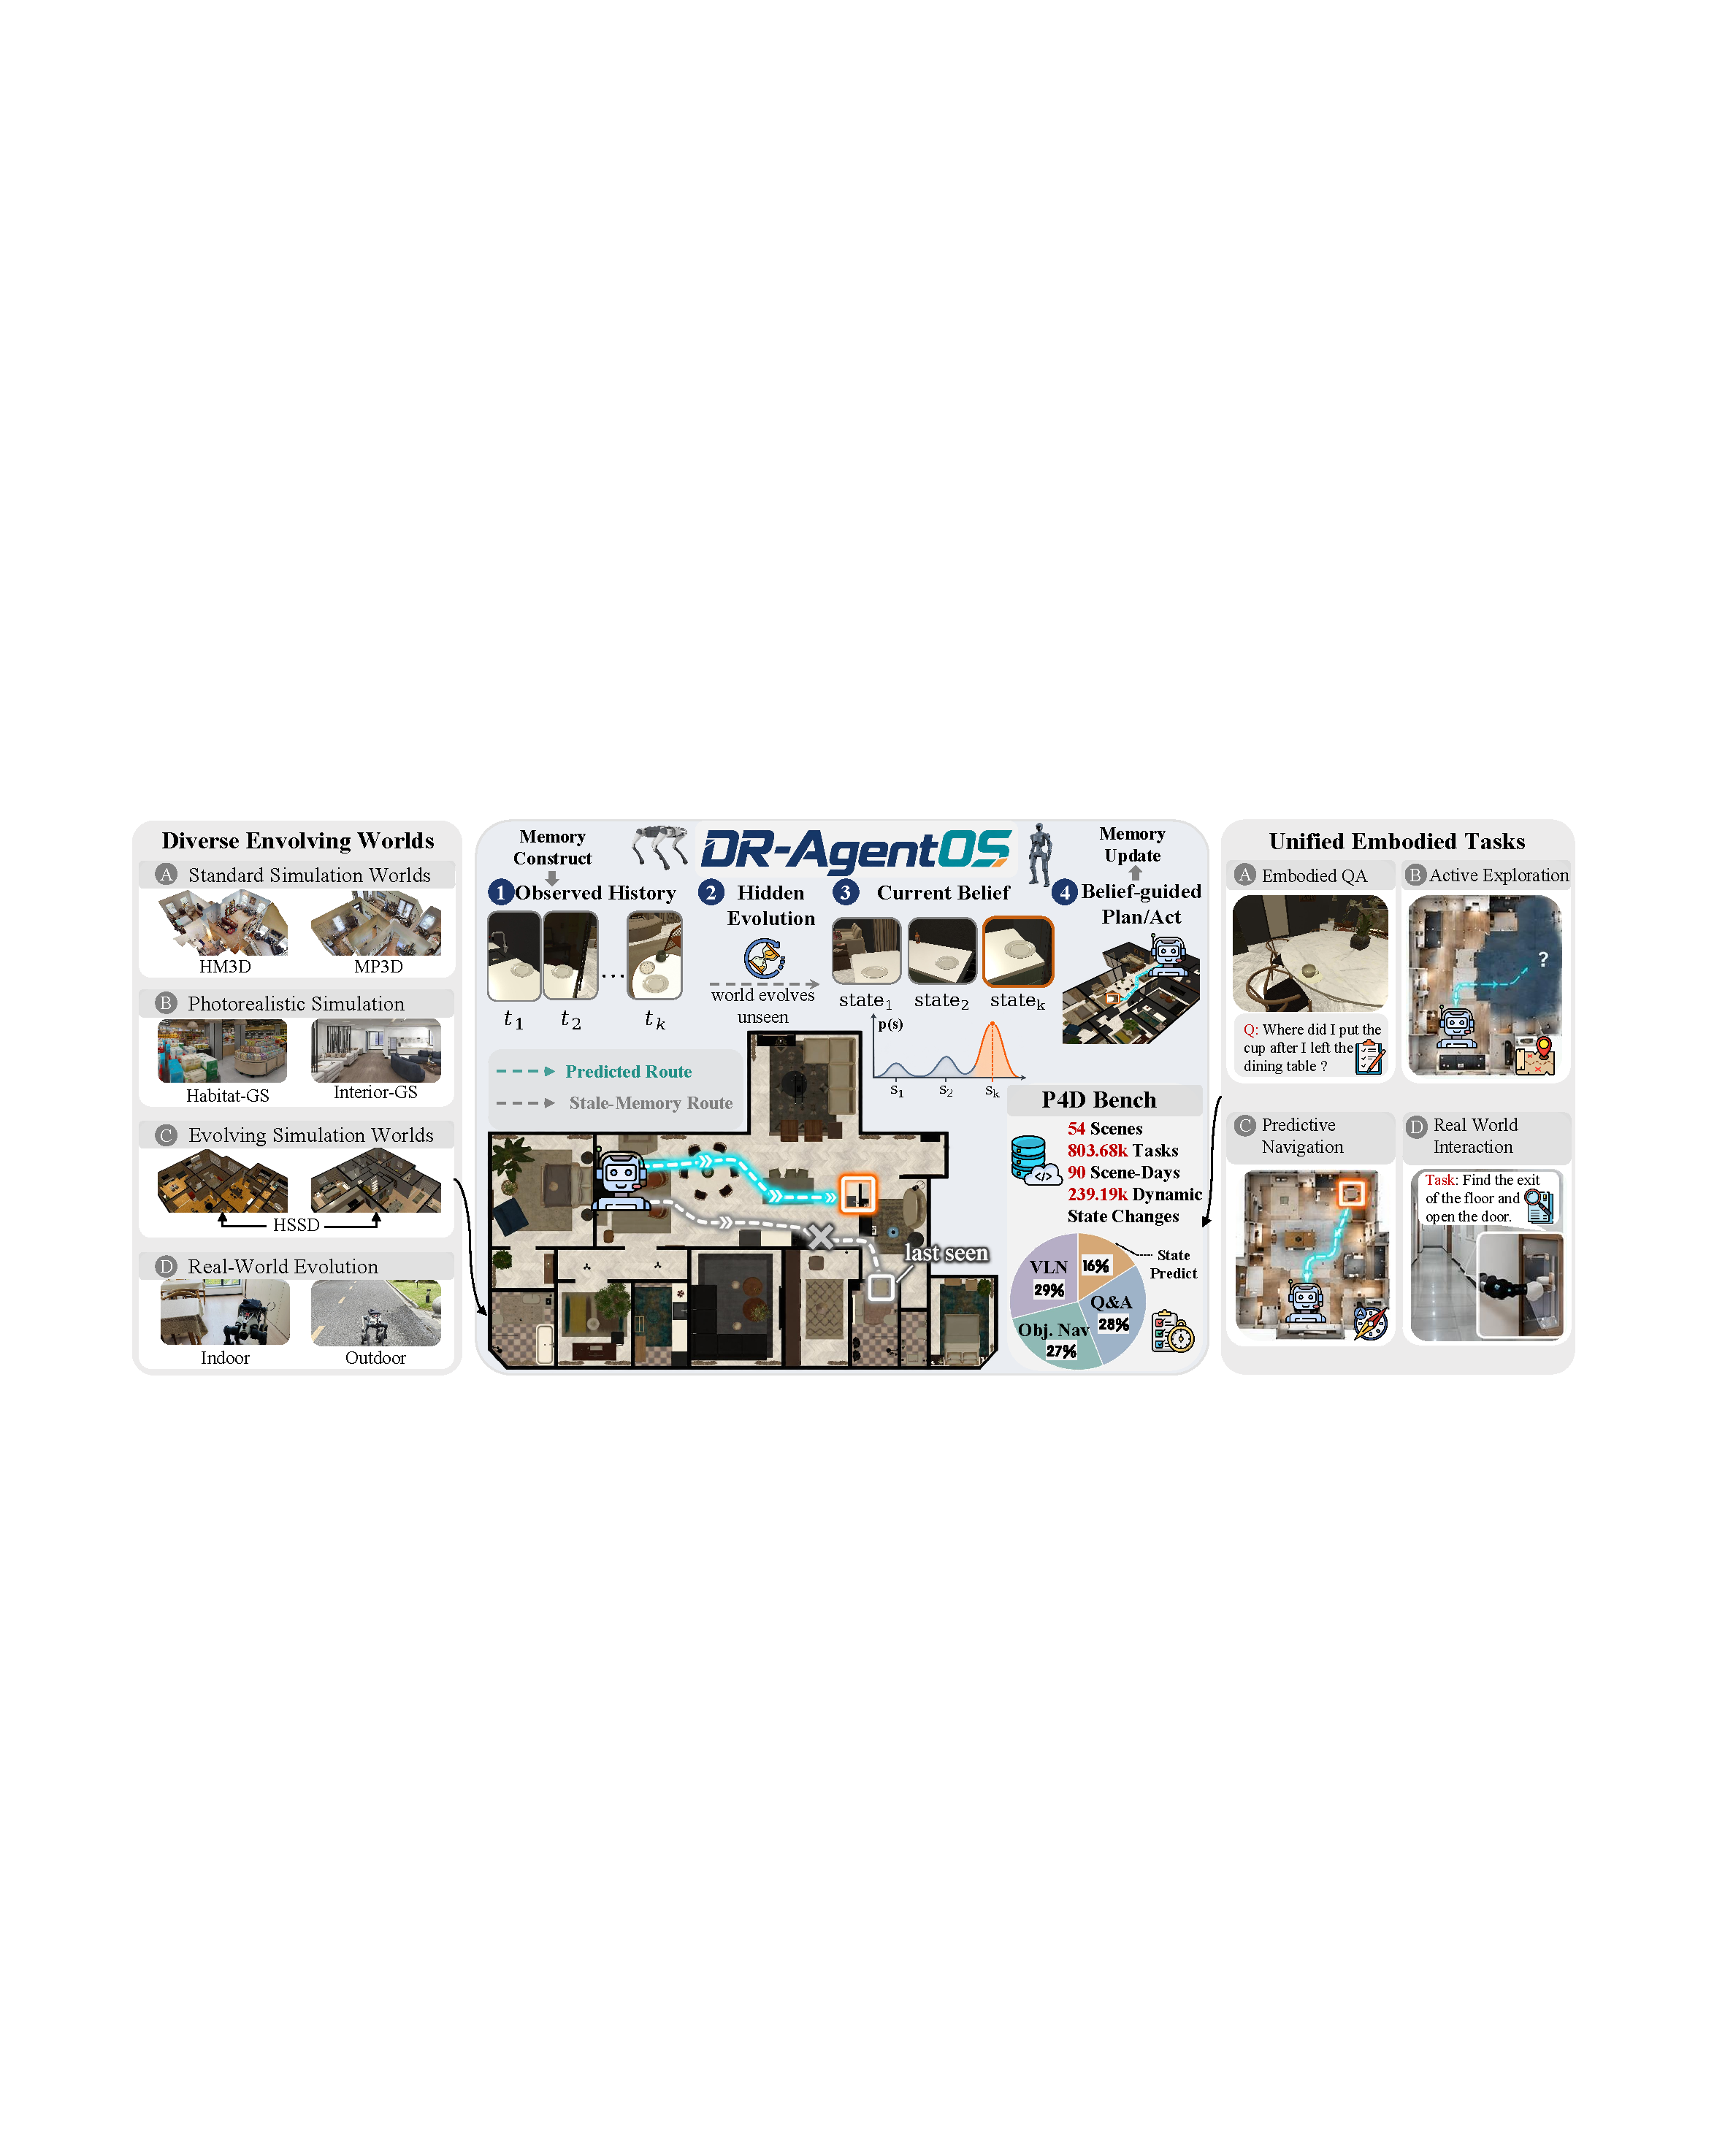
\includegraphics[width=\textwidth]{figures/overview.pdf}
    \caption{Overview of \evolvingworldnav{} for predictive embodied reasoning and action in evolving worlds.}
    \label{fig:evolvingworldnav_overview}
\end{figure}

\section{Introduction}
\label{sec:introduction}

Object navigation asks an embodied agent to find an instance of a requested category from egocentric observations. Progress in semantic mapping and foundation-model reasoning has made this problem increasingly tractable in static environments \citep{chaplot2020objectnav,huang2023vlmaps,gu2024conceptgraphs}. A household robot deployed over weeks, however, rarely acts in the scene that it originally mapped. A mug last observed beside the sink may have moved to a desk after breakfast; keys may alternate between a shelf and a bag; and a rarely moved appliance may remain exactly where it was. In each case, the agent has a valid historical observation but an uncertain current navigation goal.

This distinction exposes a limitation of conventional embodied memory. Most spatial memories answer \emph{where was the object observed?}; navigation requires \emph{where is it likely to be now?} More importantly, a predictive answer should not be consumed as a static waypoint. Travelling takes time, candidate locations differ in inspection cost and visibility, and a failed inspection is new evidence. A useful memory must therefore support a closed loop: retrieve relevant history, propagate it to the query time, select a cost-effective location, observe, update the belief, and replan.

Several recent lines of work approach parts of this problem. Dynamic scene memories update object states after new observations \citep{liu2024dynamem,kurenkov2023dynamic}; predictive scene graphs estimate the persistence or re-emergence of time-varying relations \citep{saavedraruiz2026predictivegraphs}; and models of household routines predict multimodal future object placements for downstream navigation \citep{patel2023homer,argenziano2026flowmaps}. Portable Object Navigation goes further by allowing a target to move while the agent travels and learning transit-aware policies \citep{dorbala2026portable}. These methods establish that dynamics matter, but leave a complementary question open: how should an agent turn its own long-term, partially observed memory into a belief that directly controls physical search and is corrected by the evidence collected along the route?

We formulate this setting as \textbf{persistent dynamic object navigation}. Before receiving a query, the agent has accumulated a timestamped 4D memory through intermittent visits. The target may undergo one or more hidden transitions after its last positive observation. At query time, the agent receives neither the current state nor the activity that caused the transition. It must find the object under a navigation budget using only causal memory, a map of candidate receptacles and viewpoints, and online RGB-D observations. Our main protocol freezes the target once the query begins to isolate the value of predictive memory; an extension allows an additional hidden transition during navigation.

We introduce \pfdnav{}, a compact predictive-memory agent for this problem. Its 4D memory maintains persistent entity identities, time-valid state versions, and observation provenance in a common 3D frame. A target-conditioned retriever exposes only the history available before the query. A lightweight continuous-time Transformer represents irregular temporal gaps and calendar periodicity. Instead of directly classifying a location, a structured head factorizes the belief into (i) the probability that the last-seen state persists and (ii) a pointer distribution over relocation candidates. This inductive bias matches the physical alternatives faced by a navigator and supports candidate sets that vary across scenes.

Prediction is coupled to action through a visibility-aware evidence update and a belief-guided controller. Concentrated beliefs support a direct first attempt; diffuse beliefs induce a probability--cost search order; and sufficiently covered negative observations suppress inspected hypotheses before replanning. The controller is identical across stable, routine-mobile, personal-habit, and irregular objects and receives no mobility label at test time. Thus, static recall, predictive navigation, and uncertainty-driven search emerge from one belief rather than from an oracle router.

To evaluate the resulting navigation problem, we introduce \pfdbench{}. Its dynamic HSSD episodes are compiled through a canonical routine representation that combines complementary signals from longitudinal activity records, real human--object interactions, and household object-state scripts. More importantly, the benchmark contains paired static, routine, and random worlds that share the scene, target, last observation, query time, candidate set, and agent start. Only the hidden transition process differs. This counterfactual construction tests whether an agent exploits temporal structure instead of object--location frequency or route-length shortcuts.

\paragraph{Contributions.}
Our contributions are threefold:
\begin{itemize}[leftmargin=5mm,itemsep=0.6mm,topsep=1mm]
    \item We formulate persistent dynamic object navigation, connecting long-term, partially observed memory to closed-loop physical search under hidden object transitions.
    \item We propose \pfdnav{}, which combines an evidence-grounded 4D memory, continuous-time history encoding, a persistence--relocation belief, and visibility-aware Bayesian correction to support direct navigation, belief-guided search, and recovery without oracle dynamics labels.
    \item We introduce \pfdbench{}, a human-trace-grounded HSSD benchmark with paired dynamic controls, instance-level mobility regimes, online replanning tasks, and cross-scene and cross-household evaluation.
\end{itemize}

\section{Related Work}
\label{sec:related_work}

\paragraph{Semantic and dynamic world models.}
Visual Language Maps attach language-aligned features to maps for open-vocabulary navigation \citep{huang2023vlmaps}, while ConceptGraphs and HOV-SG organize entities in open-vocabulary 3D scene graphs \citep{gu2024conceptgraphs,werby2024hovsg}. These representations support spatial retrieval but principally describe a scene state. DynaSLAM removes dynamic content during mapping \citep{bescos2018dynaslam}; lifelong semantic mapping and DynaMem instead update maps as environments evolve \citep{narayana2020lifelong,liu2024dynamem}. Other work represents time-indexed 3D content or human-centered events \citep{gorlo2025daaam,bartoli2026gesto}. \dragentos{} builds on these lines by treating temporal validity, stable identity, and source evidence as a shared service used by reasoning and execution.

\paragraph{Embodied agents and memory.}
SayCan grounds language-model decisions in skill affordances, and PaLM-E injects embodied observations into a multimodal language model \citep{ahn2022saycan,driess2023palm}. Recent systems increasingly combine foundation models, spatial memory, and tool use \citep{zhou2026holoagent,tian2026abot,wang2026thea,li2026agenticnav,xin2026agentvln}. Long-term-memory and EQA benchmarks test whether stored experience supports later reasoning \citep{majumdar2024openeqa,wang2026explore}. Our focus is the systems boundary between these components: the controller may interpret goals and choose tools, but mapping, execution, verification, and evidence-gated commit retain authority over physical facts.

\section{Predictive 4D Belief Navigation}
\label{sec:method}

\evolvingworldnav{} maintains a current-state belief from timestamped 3D histories
and RGB-D evidence; \pfdnav{} separates persistence from relocation
(\cref{fig:p4dnav_method}).

\subsection{Problem Formulation}
\label{sec:problem}

An environment contains a navigable space $\mathcal X$, entities $\mathcal O$,
and candidate states $\mathcal C_o$ with inspection viewpoints. Before query
time $t_q$, the agent has only the causal history
\begin{equation}
\mathcal H_{\leq t_q}=\{(I_k,D_k,\xi_k,t_k)\mid t_k\leq t_q\},
\end{equation}
where $I_k,D_k,\xi_k$ denote RGB, depth, and camera pose. The hidden state lies in
$\widetilde{\mathcal C}_o=\mathcal C_o\cup\{\mathrm{unknown}\}$; later
out-of-view transitions are also hidden.

Given a target, initial pose $x_0$, memory, and action budget, the agent observes
$z_j$ after acting and must stop at a valid target viewpoint. It optimizes
\begin{equation}
\pi^*=\arg\max_{\pi}\;\mathbb E_{\pi}\!\left[
\mathbb I(\mathrm{success})-\lambda_d L-\lambda_n N_{\mathrm{inspect}}
\right],
\label{eq:objective}
\end{equation}
where $L$ is the travel distance and $N_{\mathrm{inspect}}$ is the inspection count.

\begin{figure}[t]
    \centering
    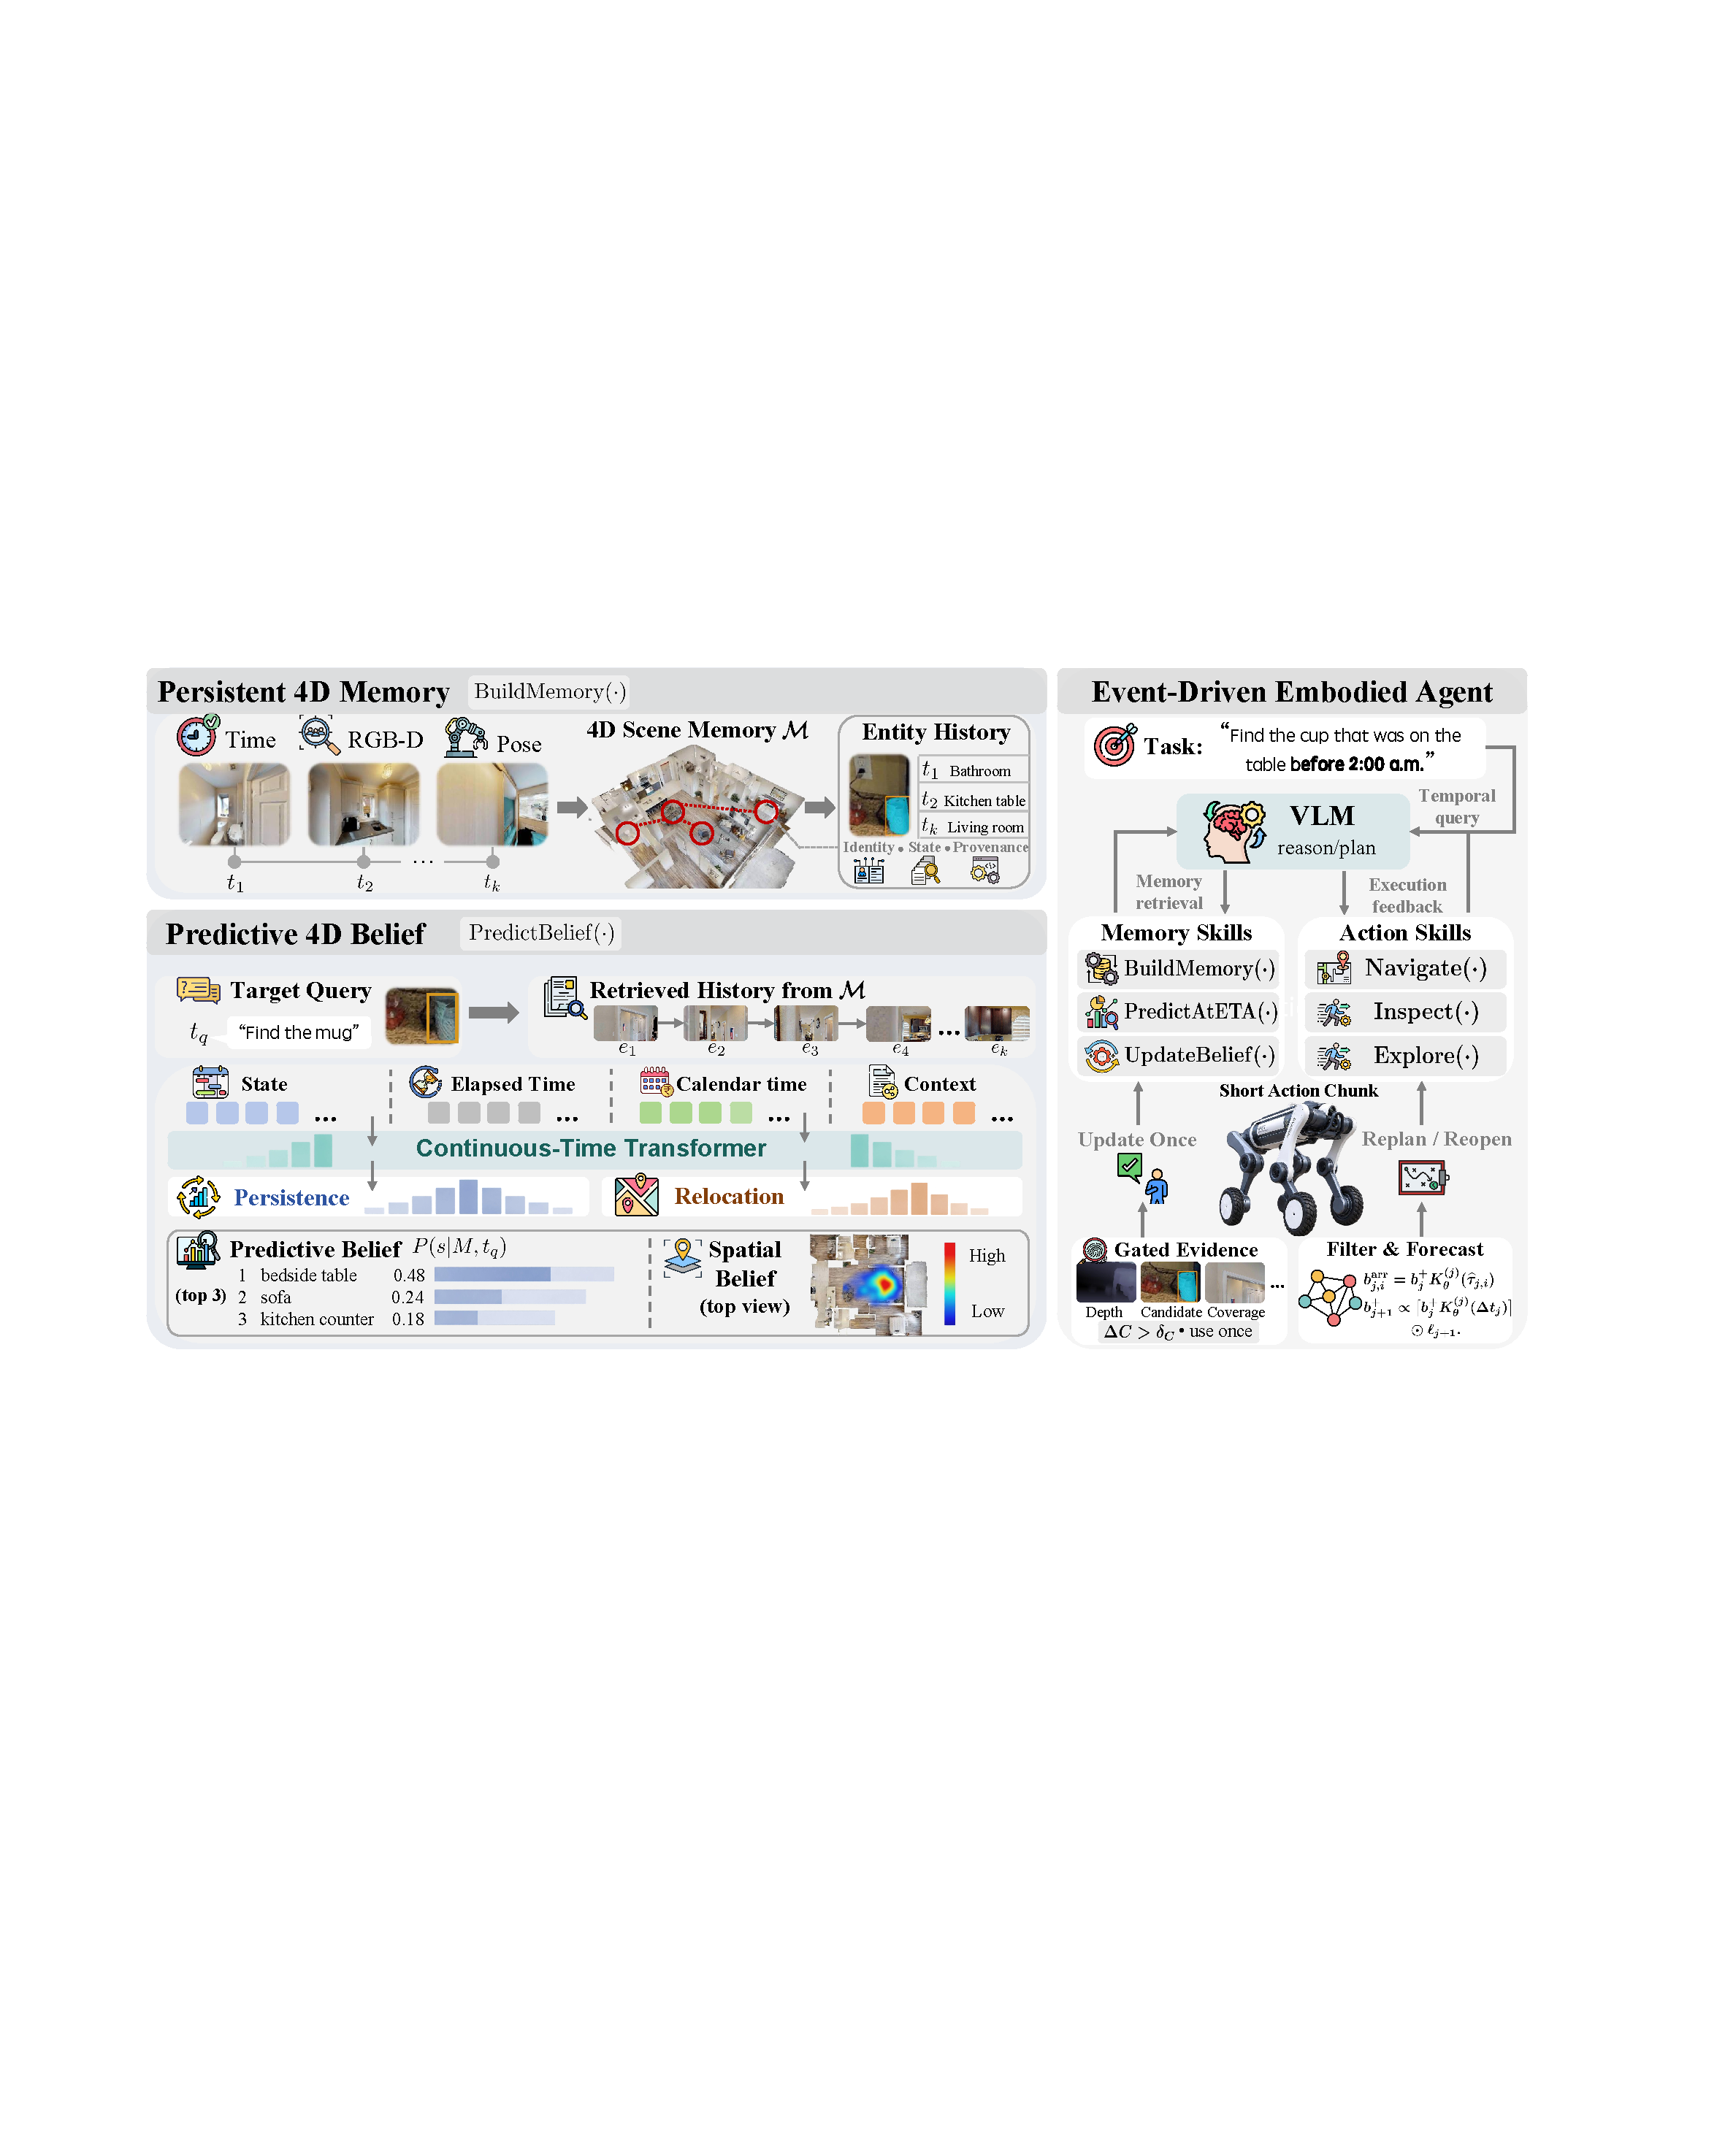
\includegraphics[width=\linewidth]{figures/method.pdf}
    \caption{\evolvingworldnav{} couples persistent 4D memory, predictive belief,
    and an embodied agent that updates and replans from stepwise evidence.}
    \label{fig:p4dnav_method}
\end{figure}

\subsection{Causal 4D Memory and History Encoding}
\label{sec:memory_encoding}
The 4D memory registers RGB-D observations in a shared frame, associates entities using
semantics, geometry, and time, and materializes versioned deltas causally:
\begin{equation}
\mathcal M_{\leq t}=\operatorname{Materialize}(\Delta\mathcal M_0,\ldots,\Delta\mathcal M_t)
=(\mathcal G_t,\mathcal V_t,\mathcal B_t),
\label{eq:memory}
\end{equation}
where $\mathcal G_t,\mathcal V_t,\mathcal B_t$ store relations, time-valid
versions, and provenance. Changes append versions without erasing history;
perception and versioning details are in \appref{app:memory-details}
\citep{liu2024grounding,ravi2025sam,radford2021learning}.

\paragraph{Target-conditioned history and continuous time.}
For target $o$, a typed query returns the most recent $K$ causal events
\begin{equation}
H_o=\{e_k=(o_k,s_k,t_k,z_k,c_k,v_k)\}_{k=1}^{K},
\label{eq:history}
\end{equation}
where $o_k,s_k,t_k,z_k$ encode entity, candidate state, time, and
$\{\mathrm{seen},\mathrm{notseen}\}$ evidence; $c_k,v_k$ encode confidence and
visibility. Related context events are causal, candidate encodings capture
function and geometry, and \texttt{unknown} absorbs unmapped states.

Each event token combines semantic, evidence, and temporal features:
\begin{align}
\mathbf x_k={}&E_o(o_k)+E_s(s_k)+E_z(z_k)+E_c(c_k)+E_v(v_k)\nonumber\\
&+\phi_{\Delta}(t_q-t_k)+\phi_{\mathrm{cal}}(t_k),
\label{eq:eventtoken}
\end{align}
where $\phi_{\Delta}$ encodes log elapsed time and $\phi_{\mathrm{cal}}$ encodes
hour and weekday. A query token specifies the target, time, and last observed state; a compact
Transformer yields
\begin{equation}
(\mathbf h_1,\ldots,\mathbf h_K,\mathbf h_q)
=\operatorname{CTTransformer}(\mathbf x_1,\ldots,\mathbf x_K,\mathbf x_q).
\label{eq:history-encoder}
\end{equation}
The encoding captures irregular intervals, evidence, and event order without hidden labels.

\subsection{Persistence--Relocation Belief}
\label{sec:belief_model}
We predict persistence at the last observed state or relocation elsewhere.
Episode validity guarantees a last positively observed state $s_{\mathrm{last}}$
(\appref{app:audit}). The persistence branch predicts
\begin{equation}
\rho_q=P(s_{t_q}^o=s_{\mathrm{last}}\mid H_o,t_q)
=\sigma(\mathbf w_{\rho}^{\top}\mathbf h_q).
\label{eq:persistence}
\end{equation}
For each alternative $i\in\widetilde{\mathcal C}_o\setminus
\{s_{\mathrm{last}}\}$, a shared pointer head computes
\begin{equation}
a_i=\frac{(W_q\mathbf h_q)^\top(W_c\mathbf g_i)}{\sqrt d}
+\psi(\mathbf h_q,\mathbf g_i),\qquad
\pi_q(i)=\frac{\exp a_i}{\sum_{u\in\widetilde{\mathcal C}_o\setminus\{s_{\mathrm{last}}\}}\exp a_u},
\label{eq:pointer}
\end{equation}
where $\mathbf g_i$ represents candidate $i$, $d$ is the projection dimension,
and $\psi$ measures learned compatibility. The prior is
\begin{equation}
b_q^-(i)=
\begin{cases}
\rho_q, & i=s_{\mathrm{last}},\\
(1-\rho_q)\pi_q(i), & i\neq s_{\mathrm{last}}.
\end{cases}
\label{eq:prior}
\end{equation}
We train with $\mathcal L_{\mathrm{state}}=-\log b_q^-(s_{t_q}^o)$ without
change labels; the normalized belief represents returns and alternatives.

\subsection{Predictive Embodied Agent}
\label{sec:agent}

A frozen VLM invokes memory, prediction, navigation, inspection, and exploration
tools. Action chunks, new coverage or evidence, ETA changes, and arrivals trigger
decision epochs. The encoder produces $\mathbf h_j$ for the row-normalized operator
\begin{equation}
[K_\theta^{(j)}(\Delta t)]_{r,u}=\operatorname{softmax}_{u}
f_\theta(\mathbf h_j,\mathbf g_r,\mathbf g_u,\phi_\Delta(\Delta t)).
\label{eq:transition-kernel}
\end{equation}
The operator shares the encoders in \cref{eq:history-encoder,eq:pointer}; a separate head
learns chronological state transitions through row-wise cross-entropy
(\appref{app:belief-control}). Initialized with $b_0^-=b_q^-$, the filter propagates after each chunk:
\begin{equation}
b_{j+1}^-=b_j^+K_\theta^{(j)}(t_{j+1}-t_j).
\label{eq:filter-predict}
\end{equation}
Thus $b_j^\pm$ denotes the current-time belief, separate from arrival forecasts.

\paragraph{Arrival-aware action selection.}
For candidate viewpoints $\mathcal W_i$, let
$d_{j,i}=d_{\mathrm{geo}}(x_j,\mathcal W_i)$ and $\widehat\tau_{j,i}$ be
the geodesic distance and estimated travel-plus-inspection time. The agent selects
\begin{equation}
i_j^*=\arg\max_{i\in\mathcal{C}_o}
\frac{
    p_{j,i}^{\mathrm{arr}}\,
    \widehat{q}_{j,i}^{\,\mathrm{new}}
}{
    d_{j,i}
    + \lambda_t \widehat{\tau}_{j,i}
    + \lambda_{\mathrm{inspect}}
},
\label{eq:planner}
\end{equation}
where $p_{j,i}^{\mathrm{arr}}$ is defined below and
$\widehat q_{j,i}^{\mathrm{new}}$ is the detection probability from newly covered
surfaces. Exploration expands the candidate set when unknown-state utility is highest.

\paragraph{Visibility-qualified measurement update.}
A posed RGB-D view can update every covered candidate. A calibrated detector estimates
$\widehat r_{j,i}=P(\mathrm{detect}\mid s_{t_j}=i,\mathbf f_{j,i})$ from
projected candidate geometry, online depth, and view features, without access to
ground-truth target masks or poses or simulator visibility flags. Given no detection,
\begin{equation}
\ell_j(i)=P(y_j=\varnothing\mid s_{t_j}=i)=
\begin{cases}
1-\widehat r_{j,i}, & i\in\mathcal C_o,\\
1, & i=\mathrm{unknown},
\end{cases}
\label{eq:negative}
\end{equation}
and the measurement posterior is
\begin{equation}
b_j^+(i)=\frac{b_j^-(i)\ell_j(i)}
{\sum_{u\in\widetilde{\mathcal C}_o}b_j^-(u)\ell_j(u)}.
\label{eq:bayes}
\end{equation}
An update uses only new surface coverage exceeding $\delta_C=0.05$, preventing
duplicate evidence from overlapping views. Dynamic reopening starts a new
time-valid round, allowing the same viewpoint to test a changed state. A verified match ends the search.

\paragraph{Posterior propagation and replanning.}
The current posterior is forecast to each candidate ETA for action selection,
without replacing the current-time filter:
\begin{equation}
b_{j,i}^{\mathrm{arr}}=b_j^+K_\theta^{(j)}(\widehat\tau_{j,i}),\qquad
p_{j,i}^{\mathrm{arr}}=b_{j,i}^{\mathrm{arr}}(i).
\label{eq:arrival-belief}
\end{equation}
Fixed-target episodes use identity dynamics; continuing evolution follows
\cref{eq:filter-predict,eq:arrival-belief}. At each epoch, the agent propagates
belief, incorporates new evidence once, forecasts arrival-time states, and replans
(\appref{app:belief-control}).

\section{P4D-Bench: Evaluating Navigation in Evolving Worlds}
\label{sec:benchmark}

\pfdbench{} couples longitudinal hidden state changes with executable embodied
episodes across \textbf{54 scenes} and \textbf{803.68k task instances}.
Unlike fixed-scene evaluation, it tests whether an agent can infer the present
from a causal history after an observation gap. Four design constraints preserve
temporal continuity, causal observability, physical executability, and controlled
dynamics: histories persist across queries, public evidence precedes the query,
placements have reachable inspection viewpoints, and paired worlds isolate the
hidden transition mechanism.

\begin{figure}[!htbp]
    \centering
    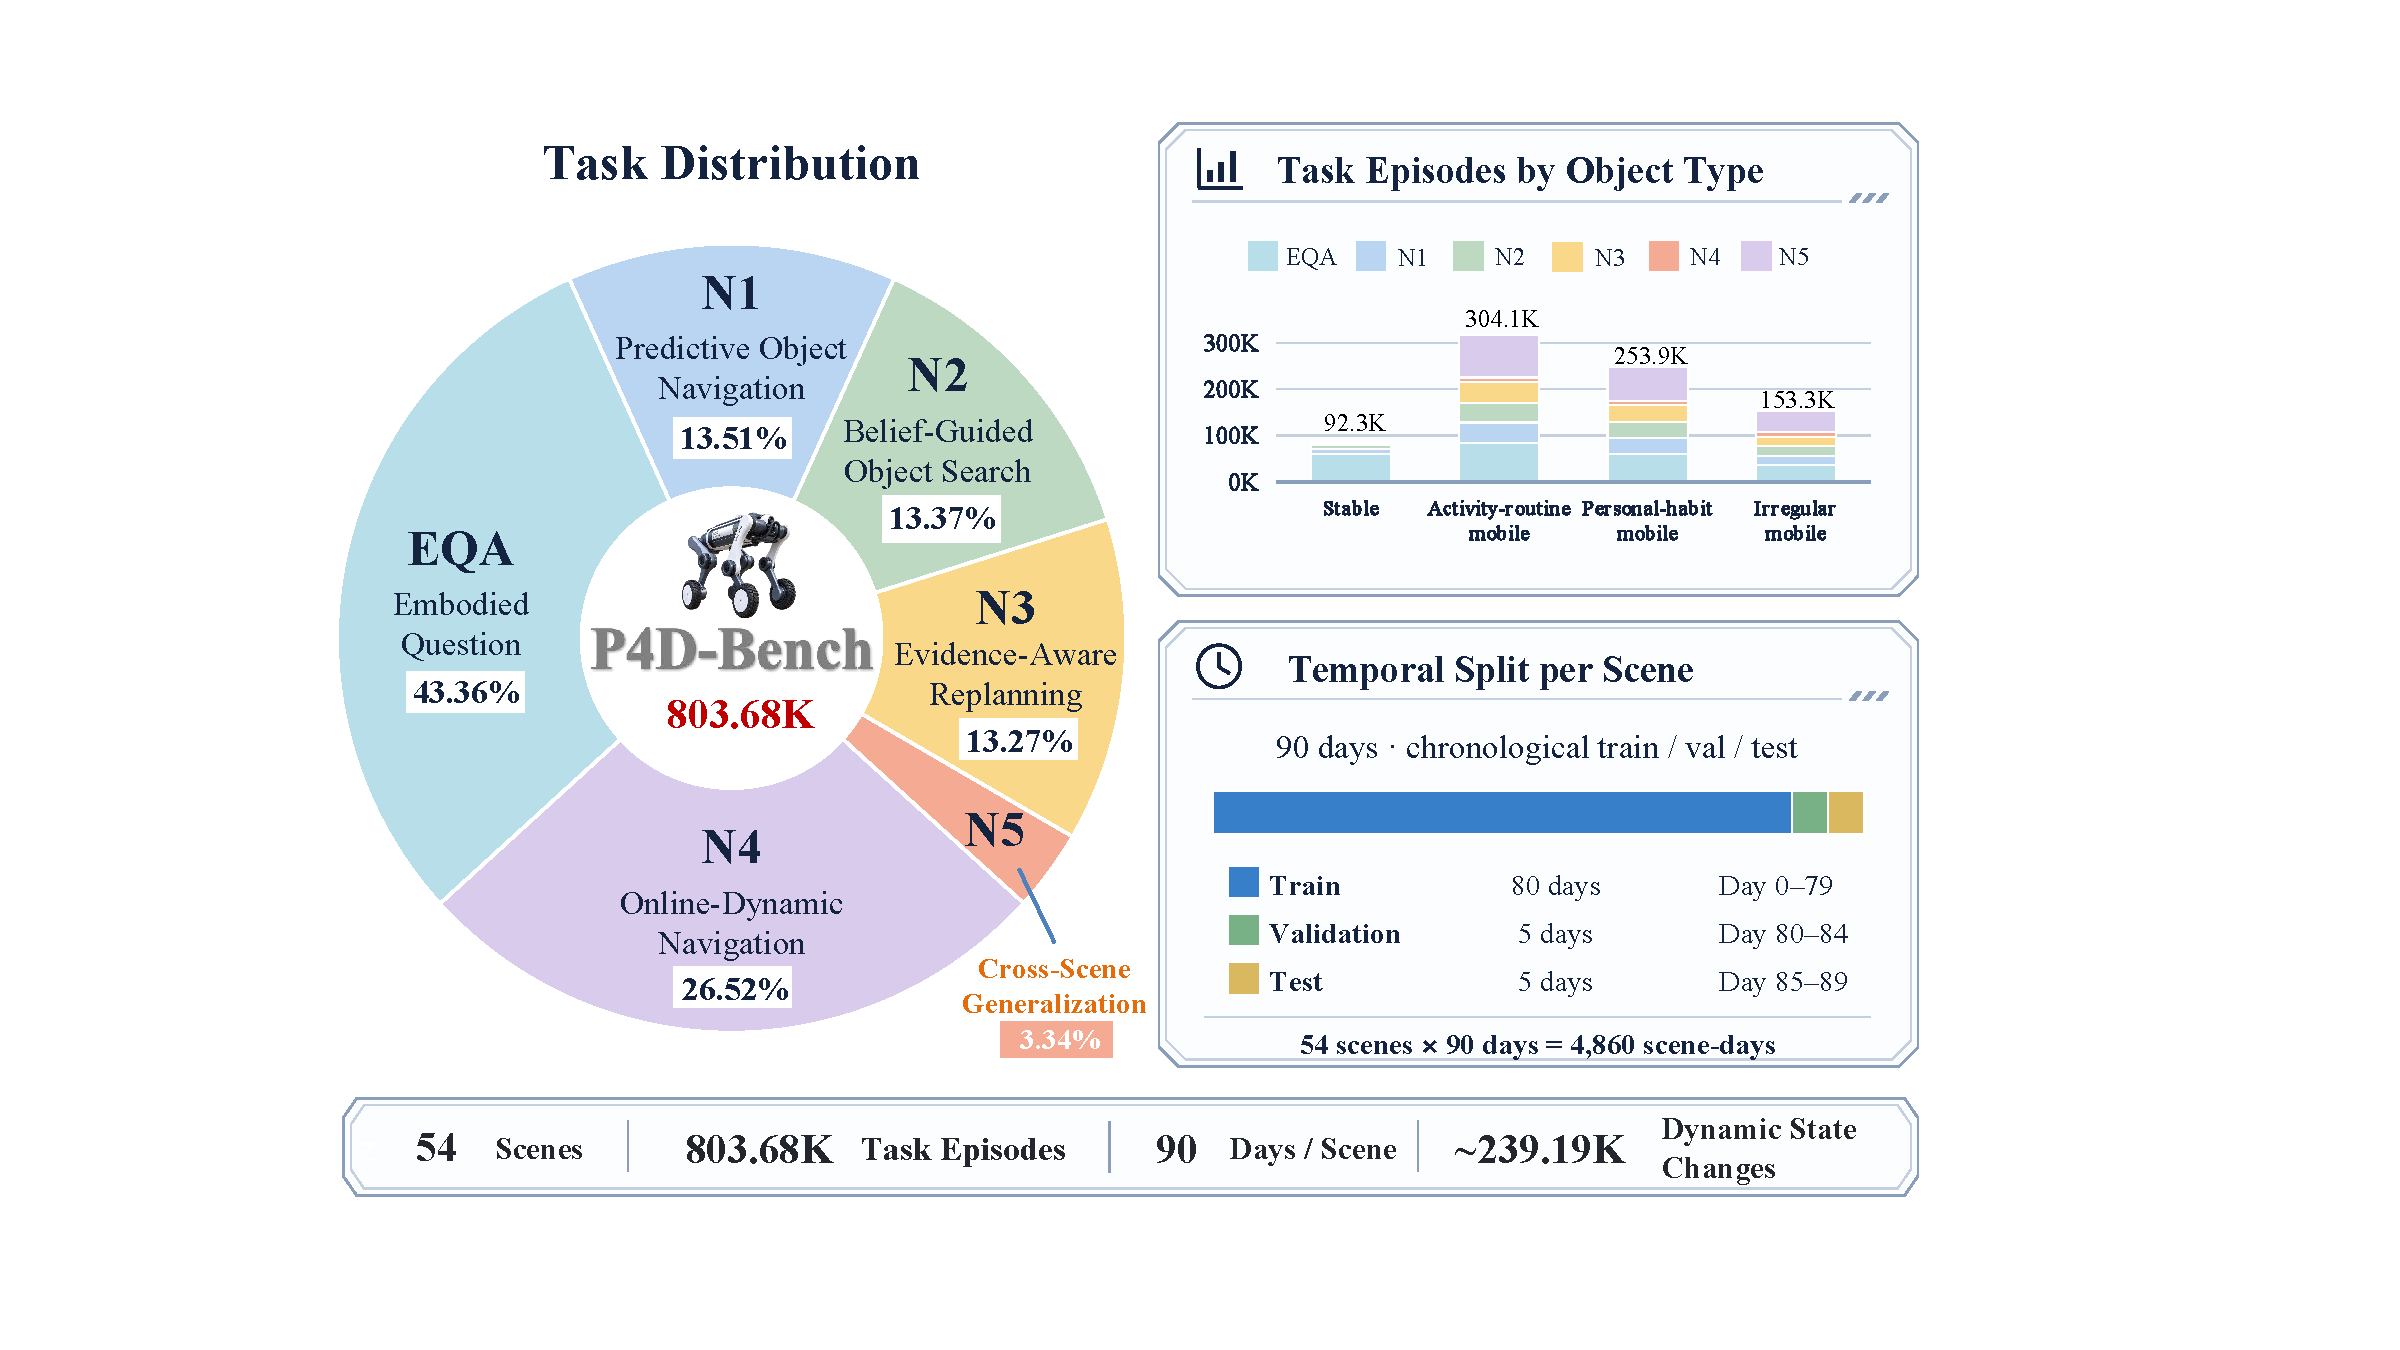
\includegraphics[width=0.80\linewidth]{figures/P4D_Benchmark.pdf}
    \caption{Overview of \pfdbench{} evaluation protocols.}
    \label{fig:p4dbench}
\end{figure}

\paragraph{Task coverage.}
The pool contains current-state prediction (16\%), object navigation (27\%),
vision-and-language navigation (29\%), and embodied question answering (28\%)
\citep{majumdar2024openeqa,sakamoto2024map}.
The experiments emphasize prediction and navigation; EQA diagnoses memory,
while the remaining annotations support broader study.
All tracks share evolving scene histories and causal evidence
(\cref{fig:p4dbench}).

\paragraph{Human-trace-grounded construction.}
We align longitudinal smart-home records from CASAS \citep{cook2013casas} and
ARAS, multi-week activity and object-location sequences from HOMER+
\citep{patel2023routine}, and action--object and placement evidence from HD-EPIC
and ParaHome \citep{perrett2025hdepic,kim2025parahome}, supplemented by
OPPORTUNITY. A common event schema links time, activity, actor context, object,
source and destination states, and provenance. These sources constrain schedules,
activity--object associations, transition timing, and placement tendencies;
trajectories are not copied into simulation. Unsupported quantities are marked
as benchmark-authored (\cref{app:world-generation}).

\begin{figure}[!htbp]
    \centering
    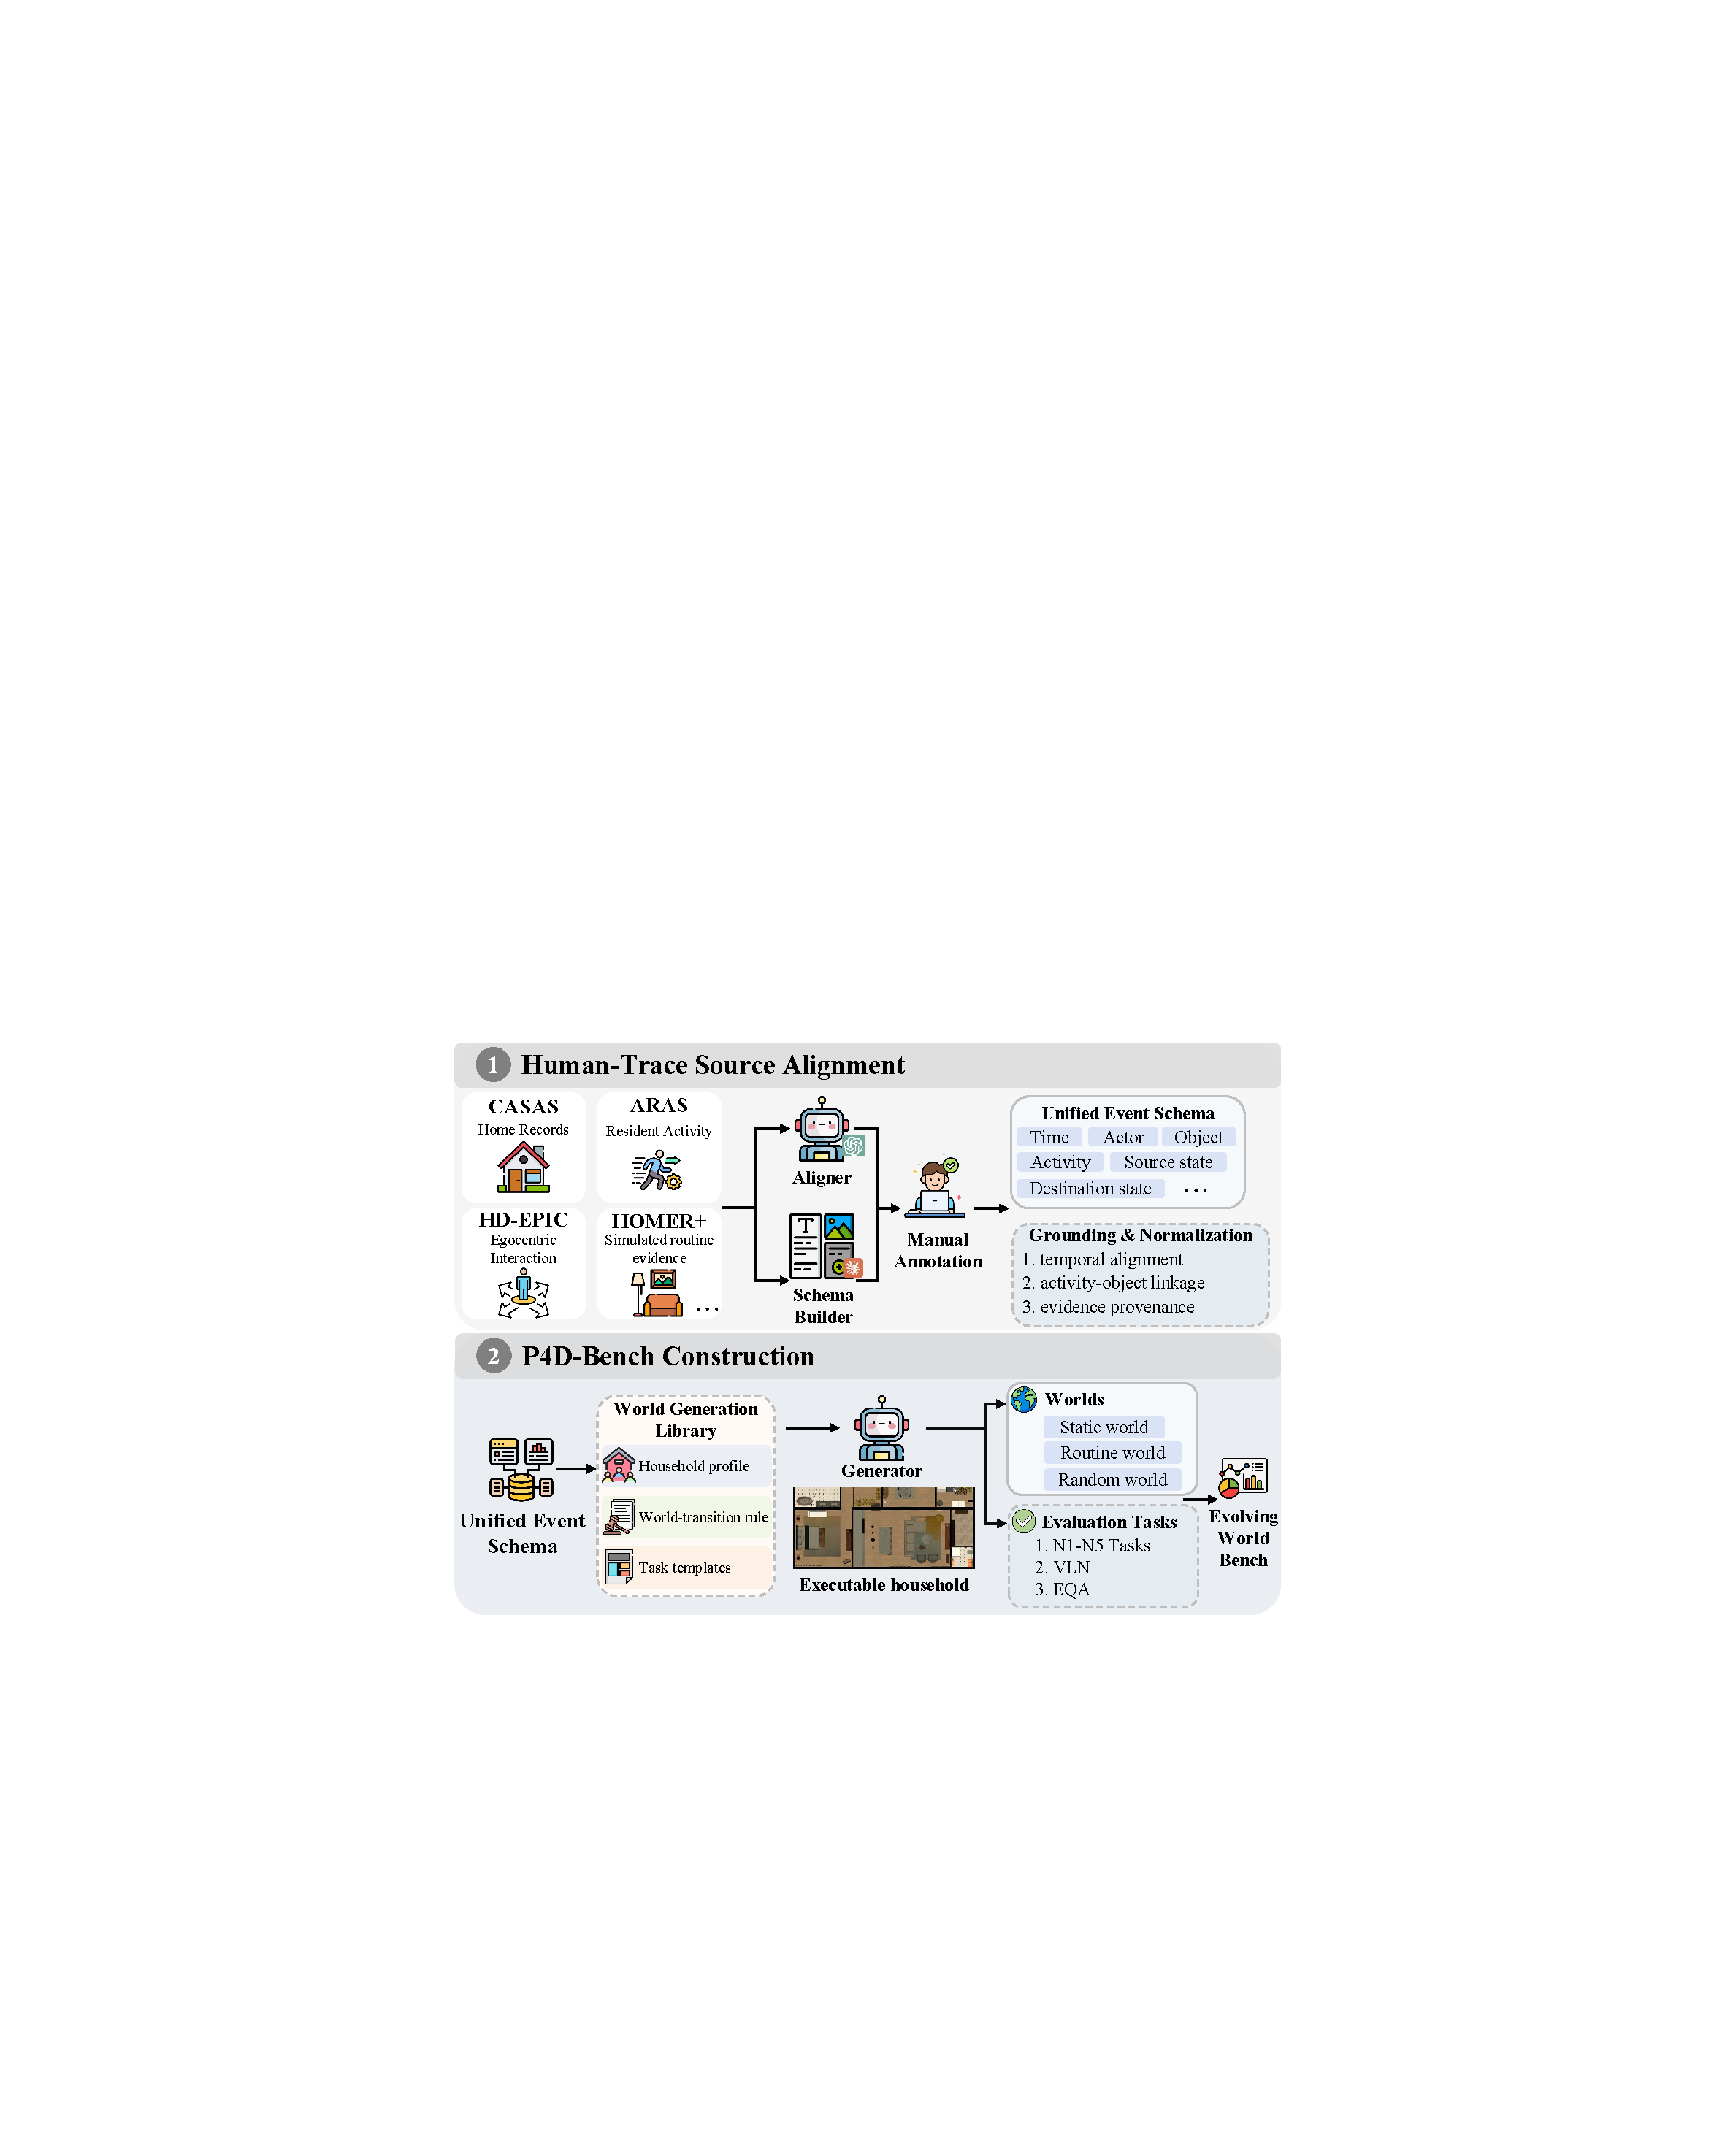
\includegraphics[width=0.80\linewidth]{figures/dataset-generate.pdf}
    \caption{Human-trace-grounded construction of \pfdbench{}.}
    \label{fig:p4dbench-generation}
\end{figure}

Across 54 HSSD scenes \citep{khanna2024hssd}, household schedules, preferences,
ownership, and placement habits are frozen while activities, resident
trajectories, and object transitions are generated chronologically
(\cref{fig:p4dbench-generation}). These persistent factors make history
informative; stochastic events and exceptions prevent deterministic scripts.
Audited histories yield 42.6 region transitions per resident-day, 6.56 relocations
per personal object-day, 52.6\% within-region relocations, and zero terminal
collisions.

\paragraph{Paired worlds.}
Targets span stable/rare, routine, personal, and irregular mobility regimes;
the labels are hidden from agents (\cref{tab:mobility-regimes}). For compatible
histories and queries, paired \emph{static}, \emph{routine}, and \emph{random}
worlds share public setup variables. Static preserves the last supported state;
routine follows the household's frozen transition process; random preserves
legal candidates and marginal movement statistics while breaking learnable
temporal dependency. Routine-specific gains therefore test historical regularity
rather than category frequency or spatial convenience.

\paragraph{Physical realization and causal observation.}
Transitions are replayed chronologically in Habitat. Each placement must be
semantically valid, collision-free, and observable from a reachable viewpoint;
recorded geometry includes geodesic cost and visibility. A robot patrol uses only
the map, time, travel cost, and its own history to collect local RGB-D snapshots
and visibility-qualified evidence. Public inputs end at $t_q$ and include
observed history, the last supported state, elapsed and calendar time, legal
candidates, and spatial context. Current states, hidden transitions, activities,
mobility labels, and oracle viewpoints remain evaluator-private.

\paragraph{Evaluation protocols.}
Prediction and navigation derive from the same target--time queries
(\cref{tab:tasks}). Prediction evaluates the current-state belief without
control. N1 permits one predicted destination (First-Go SR); N2 permits
belief-guided search (Search SR and cost); N3 updates the belief after inspection
(Recovery SR); and N4 advances the world during execution (Online Recovery SR).
N5 applies these protocols to held-out scenes and households. The main navigation
protocol freezes the target after the query. Methods receive identical public
observations, candidates, geometry, starts, controllers, and budgets; only
memory, belief, and resulting decisions differ.

\paragraph{Splits and audits.}
Complete temporal sequences are split together; held-out homes test cross-scene
generalization, and paired variants and near-duplicate transition groups remain
in the same split. Audits check future timestamps, hidden fields, answer-correlated
identifiers, duplicate groups, paired-world consistency, physical validity,
reachable goals, and patrol independence from hidden state. Results are
stratified by mobility, transition class, staleness, spatial difficulty, and split.
Construction details, task definitions, and metric implementations are provided
in \cref{app:benchmark-protocol,app:benchmark-extended-design}.
\FloatBarrier

\section{Experiments}
\label{sec:experiments}
\label{sec:setup}
\label{sec:baselines}
\label{sec:metrics}

\paragraph{Setup.}
We evaluate current-state prediction, First-Go navigation, search, and recovery
on \pfdbench{}, with FindingDory and GOAT-Bench testing broader memory use.
Within each comparison, methods share perception, legal candidates, inspection
viewpoints, low-level control, and action budgets; the VLM controller remains
frozen. Baselines cover open-vocabulary/lifelong navigation, structured memory,
and predictive world models. Released policies retain their native protocol;
otherwise, memory or prediction modules use the shared controller.
Prediction is scored by Top-1, MRR, and NLL. First-Go SR permits inspection of
only the initial candidate; Search SR measures eventual success; Recovery SR is
conditioned on an incorrect first prediction. SPL and inspection/travel costs
measure efficiency. Protocols, baseline adaptations, additional environments,
and metric definitions are detailed in
\cref{app:experimental-setup,app:baselines,app:metrics,app:extended-setup}.

\subsection{Main Results}
\label{sec:results}

\paragraph{Comparison across embodied benchmarks.}

\begin{table*}[!htbp]
\caption{Cross-benchmark comparison (\%; best values in bold).
For \evolvingworldnav{}, $\pm$ denotes the standard deviation over five seeds.}
\label{tab:crossbench}
\centering
\scriptsize
\setlength{\tabcolsep}{4.0pt}
\resizebox{\textwidth}{!}{%
\begin{tabular}{lcccccccc}
\toprule
& \multicolumn{2}{c}{\textbf{FindingDory}} &
\multicolumn{3}{c}{\textbf{GOAT-Bench}} &
\multicolumn{3}{c}{\textbf{\evolvingworldbench{}}}\\
\cmidrule(lr){2-3}\cmidrule(lr){4-6}\cmidrule(lr){7-9}
\textbf{Method} & \textbf{HL-SR $\uparrow$} & \textbf{HL-SPL $\uparrow$} &
\textbf{SR $\uparrow$} & \textbf{SPL $\uparrow$} &
\textbf{Repeat-SR $\uparrow$} & \textbf{First-Inspection SR $\uparrow$} &
\textbf{Search SR $\uparrow$} & \textbf{SPL $\uparrow$}\\
\midrule
\rowcolor{tblnav}\multicolumn{9}{c}{Open-vocabulary and lifelong navigation}\\
VLFM \citep{yokoyama2024vlfm} & 13.42 & 10.86 & 15.79 & 5.45 & 11.82 & 20.65 & 28.36 & 24.67\\
ZSON \citep{majumdar2022zson} & 27.89 & 21.81 & 29.64 & 2.45 & 16.37 & 26.84 & 32.13 & 28.55\\
FindingDory Agent \citep{yadav2025findingdory} & \paperreported{52.44} & \na & \na & \na & \na & \na & \na & \na\\
LagMemo GLUE \citep{zhou2025lagmemo} & 32.79 & 23.25 & 20.61 & 1.74 & 11.27 & 30.18 & 42.27 & 33.82\\
\midrule
\rowcolor{tblmemory}\multicolumn{9}{c}{Structured spatio-temporal memory}\\
HOV-SG \citep{werby2024hovsg} & 21.47 & 15.20 & 28.37 & 2.23 & 12.38 & 36.46 & 52.32 & 40.61\\
DynaMem \citep{liu2024dynamem} & 30.30 & 22.78 & 14.54 & 1.71 & 15.79 & 45.33 & 71.94 & 56.83\\
\midrule
\rowcolor{tblpredict}\multicolumn{9}{c}{Predictive world and state modeling}\\
SLaTe-PRO \citep{patel2023routine} & 18.18 & 14.53 & 9.41 & 0.99 & 6.38 & 13.00 & 36.33 & 26.37\\
SGM+NEP \citep{kurenkov2023dynamic} & 34.20 & 19.48 & 10.67 & 1.64 & 2.56 & 27.26 & 41.82 & 37.00\\
FlowMaps \citep{argenziano2026flowmaps} & 13.03 & 10.24 & 25.07 & 1.32 & 7.25 & 14.33 & 32.67 & 17.35\\
PredictiveGraphs \citep{saavedraruiz2026predictivegraphs} & 24.24 & 13.50 & 10.27 & 1.80 & 7.48 & 36.18 & 43.67 & 40.36\\
\midrule
\rowcolor{tblours} & \textbf{53.22} & \textbf{38.83} &
\textbf{35.43} & \textbf{12.98} & \textbf{19.31} & \textbf{61.32} &
\textbf{86.18} & \textbf{70.15}\\
\rowcolor{tblours}\multirow{-2}{*}{\textbf{\evolvingworldnav{} (ours)}} & $\pm 3.87$ & $\pm 2.43$ & $\pm 2.16$ &
$\pm 0.92$ & $\pm 0.68$ & $\pm 3.235$ & $\pm 2.07$ & $\pm 1.74$\\
\bottomrule
\end{tabular}
}
\vspace{1pt}

\parbox{\textwidth}{\scriptsize
\textsuperscript{PR} Scores reported in the cited papers under their native
protocols. Unmarked baseline scores are from our reproductions under the
method-preserving protocol in
\appref{app:experimental-setup}.}
\end{table*}

\evolvingworldnav{} consistently improves the reported metrics across
FindingDory, GOAT-Bench, and \evolvingworldbench{}. On the
\evolvingworldbench{} N1--N5 suite, First-Inspection SR increases from
45.33\% with DynaMem to 61.32\%, and Search SR increases from 71.94\% to 86.18\%.
These results show that arrival-time prediction and en-route evidence improve
success at the first fully covered inspection, while retained hypotheses support
recovery. The gains on FindingDory and GOAT-Bench show that predictive memory
remains effective beyond the proposed evolving-world setting.

\paragraph{Online navigation under execution-time dynamics.}
\Cref{fig:p4d_case_study} shows how a routine-conditioned belief avoids an
outdated last-seen location. To evaluate the closed loop under realized target
motion, \cref{tab:n4-online} reports the N4 subset in which the target changes
location after the query and before termination. Episodes that permit motion
but contain no target transition are excluded from this comparison.

\begin{figure}[!t]
    \centering
    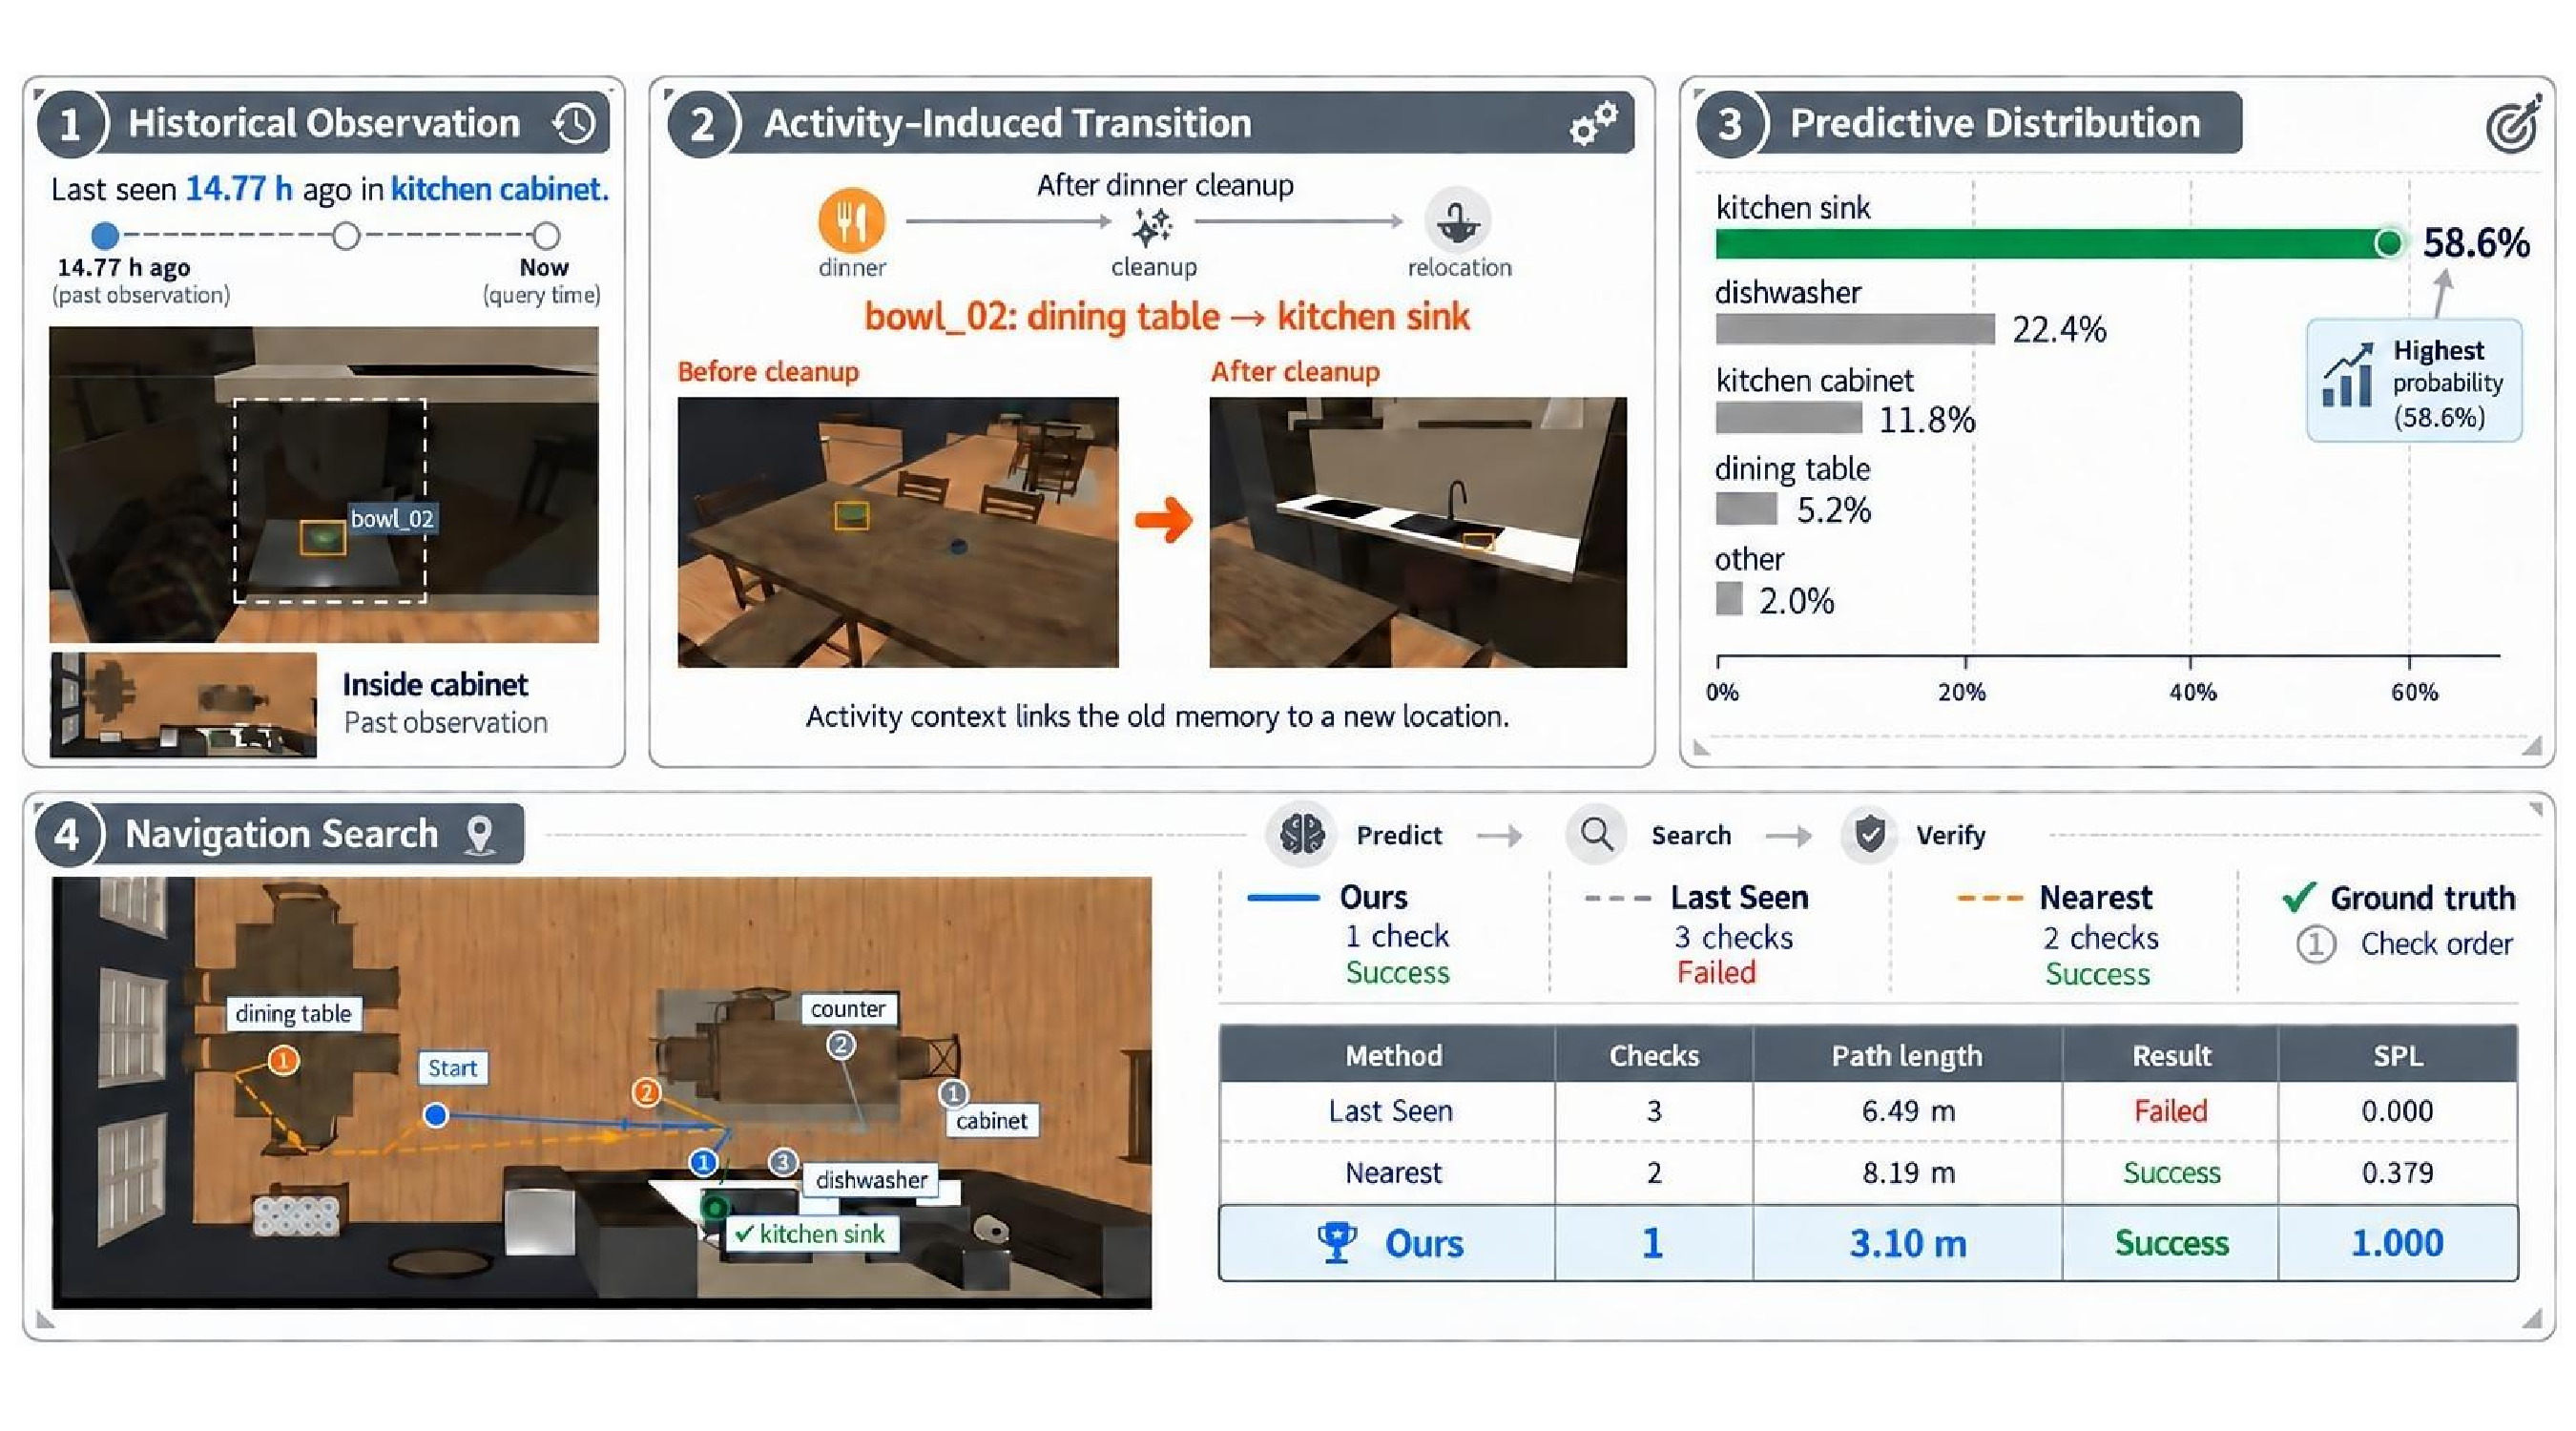
\includegraphics[width=\linewidth]{figures/P4D_CaseStudy.pdf}
    \caption{Predictive, last-seen, and nearest-first search on \evolvingworldbench{}.}
    \label{fig:p4d_case_study}
\end{figure}

\begin{table*}[!t]
\centering
\caption{Online-dynamic navigation on N4 episodes with target motion during execution.
Success rates are reported in \%; excess distance is reported in m.}
\label{tab:n4-online}
\scriptsize
\setlength{\tabcolsep}{8pt}
\begin{tabular}{lcccc}
\toprule
\textbf{Method} & \textbf{Dynamic SR $\uparrow$} &
\makecell{\textbf{Online Recovery}\\\textbf{SR $\uparrow$}} &
\makecell{\textbf{Excess Distance}\\\textbf{(m) $\downarrow$}} &
\makecell{\textbf{Revisit Success}\\\textbf{$\uparrow$}}\\
\midrule
SLaTe-PRO \citep{patel2023routine} & 34.7 & 21.5 & 18.9 & 8.7\\
SGM+NEP \citep{kurenkov2023dynamic} & 41.3 & 27.8 & 15.6 & 12.4\\
FlowMaps \citep{argenziano2026flowmaps} & 29.6 & 18.9 & 22.4 & 6.5\\
PredictiveGraphs \citep{saavedraruiz2026predictivegraphs} & 46.8 & 36.7 & 13.2 & 18.9\\
\rowcolor{tblours}\textbf{\evolvingworldnav{} (ours)} &
\textbf{65.2} & \textbf{58.7} & \textbf{8.4} & \textbf{32.6}\\
\bottomrule
\end{tabular}
\end{table*}

Relative to PredictiveGraphs, \evolvingworldnav{} improves Dynamic SR by 18.4
percentage points and Online Recovery SR by 22.0 percentage points, reduces
excess distance by 4.8\,m, and increases Revisit Success by 13.7 percentage points.
These results directly test the contribution of execution-time updates:
current-time propagation and time-valid evidence rounds allow the agent to
recover after a target moves, while candidate reopening allows productive
revisits to previously inspected locations.

\begin{wraptable}[7]{r}{0.63\linewidth}
\vspace{-0.7\baselineskip}
\caption{Primary LYNX M20 search results.}
\label{tab:real-main}
\centering
\scriptsize
\setlength{\tabcolsep}{2.2pt}
\resizebox{\linewidth}{!}{%
\begin{tabular}{@{}lrrrrrr@{}}
\toprule
Method &
\makecell{First-Inspection\\SR $\uparrow$} &
\makecell{Search\\SR $\uparrow$} &
\makecell{Recovery\\SR $\uparrow$} &
\makecell{Dist.\\(m) $\downarrow$} &
\makecell{Time\\(s) $\downarrow$} &
\makecell{Inspect.\\$\downarrow$} \\
\midrule
Last Seen + Search & 17.2 & 26.6 & 12.8 & 56.2 & 284 & 2.19 \\
Time Frequency & 21.9 & 31.3 & 14.0 & 52.9 & 277 & 2.05 \\
Retrieval + Reasoning & 26.6 & 37.5 & 17.1 & 50.3 & 281 & 2.03 \\
\rowcolor{tblours}\textbf{\evolvingworldnav{}} &
\textbf{34.4} & \textbf{48.4} & \textbf{24.3} &
\textbf{43.8} & \textbf{248} & \textbf{1.84} \\
\bottomrule
\end{tabular}%
}
\end{wraptable}

\paragraph{Generalization and physical deployment.}
Across five simulation environments, \evolvingworldnav{} achieves the highest
scores on seven of ten metrics (\cref{tab:domains}). In 64 matched M20 trials,
it improves both success and efficiency (\cref{tab:real-main}); details are in
\appref{app:real-world-eval}.

These evaluations show improvements in initial destination selection across
benchmarks, recovery under execution-time motion in N4, and path length and
inspection count in robot trials using the same belief interface. The
consistent gains across these settings argue against benchmark-specific
exploration or a stronger controller as the sole explanation.

\subsection{Ablation Studies}
\label{sec:ablations}

\paragraph{Core components.}
\begin{figure}[H]
    \centering
    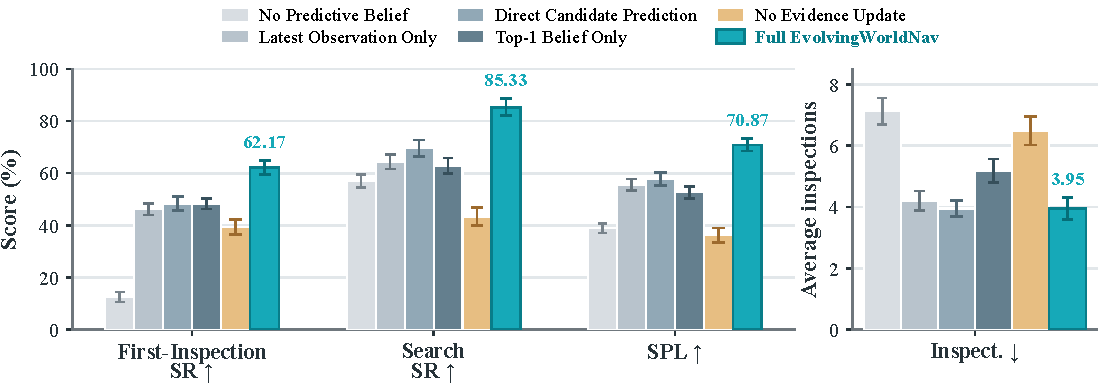
\includegraphics[width=\columnwidth]{figures/core_component_ablation_grouped.pdf}
    \caption{Core component ablation. Error bars show standard deviations over five seeds.}
    \label{fig:module_ablation}
\end{figure}

The full agent achieves 62.17\% First-Inspection SR, 85.33\% Search SR, and
70.87\% SPL with 3.95 inspections (\cref{fig:module_ablation}). Removing predictive
belief lowers First-Inspection SR to 12.51\%, while Latest Observation Only
reduces Search SR by 20.91 percentage points. Temporally persistent history
guides both initial destination selection and recovery.
Direct candidate prediction reduces First-Inspection SR and Search SR by
13.84 and 15.75 percentage points, respectively, supporting the
persistence--relocation factorization. Top-1-only search reduces Search SR by
22.41 percentage points; removing evidence updates reduces it by 42.02
percentage points and increases the inspection count to 6.48. Retaining
alternative hypotheses enables recovery, while evidence updates turn new views
into route changes; neither a better single prediction nor a larger search
budget explains these gains. No Evidence Update uses the same predictor, so its
performance gap isolates the action-time filter from offline state classification gains.


\begin{wraptable}{r}{0.64\linewidth}
\vspace{-0.7\baselineskip}
\caption{Current-state prediction on temporal and LOSO splits.}
\label{tab:predictors}
\centering
\scriptsize
\setlength{\tabcolsep}{2.3pt}
\resizebox{\linewidth}{!}{%
\begin{tabular}{lrrrrrr}
\toprule
& \multicolumn{3}{c}{Temporal} & \multicolumn{3}{c}{LOSO}\\
\cmidrule(lr){2-4}\cmidrule(lr){5-7}
Predictor & Top-1 $\uparrow$ & MRR $\uparrow$ & NLL $\downarrow$
& Top-1 $\uparrow$ & MRR $\uparrow$ & NLL $\downarrow$\\
\midrule
Last Seen & 0.00 & 0.1699 & 3.4011 & 50.00 & 0.5850 & 1.8825\\
Time Frequency & 33.85 & 0.5462 & 1.8400 & 49.53 & 0.6166 & 1.6455\\
Direct Transformer & 34.16 & 0.5586 & 1.7292 & 51.71 & 0.6884 & 1.3157\\
Shared semantic prior & 36.02 & 0.5957 & 1.5766 & 59.47 & 0.7462 & 1.0448\\
\rowcolor{tblours} & \textbf{38.24} & \textbf{0.5971} & \textbf{1.4925}
& \textbf{61.18} & \textbf{0.7523} & \textbf{0.9778}\\
\rowcolor{tblours}\multirow{-2}{*}{\textbf{Ours}}
& $\pm1.42$ & $\pm0.0291$ & $\pm0.0867$
& $\pm1.53$ & $\pm0.0176$ & $\pm0.0228$\\
\bottomrule
\end{tabular}%
}
\end{wraptable}

\paragraph{Prediction and controller robustness.}
Compared with the Direct Transformer, our predictor improves Top-1 by 4.08 and
9.47 percentage points and reduces NLL by 0.2367 and 0.3379 on the temporal and
LOSO splits, respectively. It also outperforms the shared semantic prior,
supporting temporal structure beyond location frequency. Larger LOSO gains
indicate transfer beyond scene-specific destination statistics, while lower NLL
provides more useful recovery alternatives. Additional ablations are in
\appref{app:experimental-results}.

\section{Conclusion}

We introduced persistent navigation in evolving worlds, where an embodied agent
must act while task-relevant changes can occur outside its view before or during
navigation. \evolvingworldnav{} closes a memory--belief--action loop: its
\pfdnav{} core separates persistence from relocation, retains uncertainty over
scene-specific candidates, converts visibility-qualified observations into
posterior evidence, and replans from the updated belief. \pfdbench{} grounds
this question in human-trace-driven HSSD histories and paired static, routine,
and random worlds. The strongest gains occur under learnable routine evolution,
while lower performance on matched random transitions defines the current
boundary of predictive benefit. Results on held-out scenes, other embodied
benchmarks, and physical robots further suggest that the belief-and-evidence
interface transfers beyond the controlled routine setting. Overall, navigation
in an evolving world requires not only remembering or predicting a destination,
but testing that belief against new physical evidence and revising action when
the world no longer supports it.

\section{Limitations}

The current formulation assumes sufficiently accurate pose and depth for cross-view association; accumulated localization error can split identities or corrupt spatial relations. Rule-based relation parsing and evidence thresholds favor auditability but cover fewer expressions than unconstrained generation. A bounded VLM can still choose the wrong legal candidate, while active verification increases latency and does not guarantee disambiguation. Memory retention also creates privacy, storage, and security risks in real deployments. Finally, the current repository lacks completed benchmark and ablation results, so no quantitative superiority claim is warranted from this draft.


\bibliographystyle{iclr2027_conference}
\bibliography{main}

\appendix
\section{Supplementary Material}

\subsection{Memory and Retrieval Records}
\label{app:records}

The persistent graph stores stable entity identifiers separately from time-varying versions. Each entity version includes its validity interval, structured attributes, confidence, feature handles, and provenance. Provenance identifies the observation time, source pose, sensor or rendered view, visual support, and content identity. The controller accesses these records through a typed memory query rather than receiving an unbounded transcript of observations.

The default retrieval service embeds descriptions, object-centric crops without rendered boxes, and full-frame context in one multimodal embedding space. Bounding-box overlays are retained only as VLM- or human-readable verification evidence; poses and world coordinates remain structured metadata and are never encoded as model-generated geometry. Near-identical similarities are tie-aware to prevent file order from producing arbitrary rank differences. The current resolver receives at most five candidates.

\subsection{Typed Tool Contract}

A tool specification contains $(n,\sigma_{\mathrm{in}},\mathcal C,\nu)$: name, structured input schema, allowed controller modes, and schema version. A call contains a unique identifier, tool name, typed arguments, and version. A result contains execution status, structured payload, evidence references, latency, and a normalized error when execution fails. Representative services cover spatiotemporal memory query, exploration-state query, semantic object retrieval, map access, route planning, navigation, inspection, and change query. The registry rejects unknown names, invalid modes, malformed arguments, and calls beyond the current budget before invoking a worker.

\subsection{Evaluation Reporting Checklist}
\label{app:protocol}

To make the completed study reproducible, the submission should report:
\begin{itemize}[leftmargin=5mm,itemsep=0.5mm]
    \item exact benchmark releases, split sizes, frame sampling, and preprocessing;
    \item exact VLM and embedding-model versions, prompts, decoding parameters, and access dates;
    \item all retrieval weights, thresholds, candidate budgets, and tie tolerances;
    \item hardware, wall-clock latency protocol, repeated-run count, aggregation, and uncertainty;
    \item baseline sources and whether values are reproduced or quoted from prior work; and
    \item per-category failures and complete ablations aligned with each claimed component.
\end{itemize}

\subsection{Submission Compliance Notes}

This source is configured for anonymous ICLR 2027 submission: \verb|\iclrfinalcopy| remains disabled, author identities and affiliations are absent, references precede the appendix, and the required AI-use statement appears before the references. The initial-submission main text must end within page 9; references and this appendix are excluded from that limit. Authors should scan figure metadata, linked repositories, acknowledgments, PDF properties, and supplementary files for identifying information before uploading. The public project URL should not be included in the anonymous manuscript unless replaced with an anonymous artifact.


\end{document}
